\documentclass[output=paper]{langsci/langscibook}
\author{Charlotte Galves\affiliation{University of Campinas} and Juanito
Avelar\affiliation{University of Campinas; Stockholm University}}
\title{Case and agreement in Brazilian Portuguese: Between Bantu and Romance}

% \chapterDOI{} %will be filled in at production

\abstract{This chapter presents some syntactic peculiarities of Brazilian
    Portuguese which differentiate it from European Portuguese and, from a
    typological point of view, put it apart in the \ili{Romance} and even in the
    \ili{Indo-European} domain. We argue that this is due to the influence of the
    African languages (mostly from the \ili{Bantu} subgroup) that were taken to
    Brazil by the slave trade during three centuries. We propose that this
    change affected T(ense), more exactly T's EPP condition, which ceased to be
    φ-dependent, with the consequence that Spec TP became an A-bar position. On
    the basis of the criteria proposed by \textcite{SheevanderWal2018}, we
    discuss the status of syntactic Case\is{case!syntactic Case} in Brazilian Portuguese and depart
    from a previous analysis that argued that, in this language, DPs could
    enter the derivation without a case feature.  In the analysis proposed in
    this chapter, Case and EPP nicely combine to account for the facts
considered.}


\begin{document}\glsresetall
\maketitle

\section{Introduction}\label{sec:key:14.1}

In this paper, we argue that Brazilian Portuguese has undergone a typological
change involving agreement and Case, under the influence of the African
languages (mostly from \ili{Bantu} subgroup) that were taken to Brazil by the slave
trade. We propose that this change affected T(ense), more exactly T’s EPP
condition, which ceased to be φ-dependent, with the consequence that SpecTP
became an A-bar position in Brazilian Portuguese.

The paper is organized as follows. In \Cref{sec:key:14.2}, we present some
syntactic peculiarities that make Brazilian Portuguese a typologically odd
language. In \Cref{sec:key:14.3}, we introduce the issue of \ili{Bantu} influence on
Portuguese during the period in which millions of Africans were taken to Brazil
by the slave trade. We show that some of the syntactic properties that
distinguish Brazilian Portuguese from the other \ili{Romance} languages are also
found in \ili{Bantu} languages. In \Cref{sec:key:14.4}, we discuss the proper
analysis of Brazilian Portuguese syntax with respect to agreement and Case,
presenting the previous proposal of \citet{AvelarGalves2011} and the discussion
of \emph{Vergnaud licensing effects} developed by \citet{SheevanderWal2018}. In
\Cref{sec:key:14.5,sec:key:14.6}, we present a proposal alternative to Avelar
and Galves’, showing some advantages and consequences for the treatment of Case
and agreement in Brazilian Portuguese. In \Cref{sec:key:14.7}, we conclude the
chapter addressing some general questions about the analysis
proposed.\footnote{Since this paper proposes both a comparative and a
    diachronic approach, we mean by European Portuguese both the language
    brought by the Portuguese colonizers in the 16th century and the language
    still spoken in Portugal. In the traditional periodization of Portuguese
    (see \citealt[73]{Castro2006} for a survey), the former is called
    \emph{Classical Portuguese} and refers to the period included between the
    first half of the 16th century and the end of the 18th century.  Although
    the grammar of Classical Portuguese and the grammar of Modern European
    Portuguese are different in many aspects, they are similar concerning the
    phenomena considered in this chapter. They can therefore, for our purposes,
    be grouped under the term “European Portuguese”.}

\section{Brazilian Portuguese: A typologically odd language}\label{sec:key:14.2}

Since the pioneering work by \citet{Pontes1987}, it has been commonly accepted
that Brazilian Portuguese exhibits properties of a topic-oriented syntax. The
more prominent property linked with this status is the so-called
\emph{topic-subject construction}, exemplified in (i) below. In addition to
this construction, Brazilian Portuguese presents other particularities
involving the subject position, agreement variation and pronouns, which are
also exemplified below.

\paragraph*{(i) Topic--verb agreement}

Brazilian Portuguese (henceforth \glsunset{BP}\gls{BP}\il{Brazilian Portuguese}), in contrast with
European Portuguese (henceforth \glsunset{EP}\gls{EP}\il{European Portuguese}), allows for
non-canonical agreement between the verb and a pre-verbal phrase that is not
the logical subject, but is generally interpreted as the topic of the sentence
(cf.
\citealt{DuarteKato2008,AvelarGalves2011,Toniette2013,MunhozNaves2012,Nunes2017}).
At least two sub-types of non-canonical agreement can be distinguished:
agreement with non-argumental locative constituents, as in \eqref{ex:key:14.1},
and agreement with non-argumental possessive constituents, as in
\eqref{ex:key:14.2}.

\ea\label{ex:key:14.1}\ili{Brazilian Portuguese}\\
    \gll \textbf{As} \textbf{ruas} \textbf{do} \textbf{centro} \textbf{não} \textbf{tão} passando carro.\\
        the.\Pl{} streets of-the downtown not are passing car\\
    \glt ‘No cars are passing through downtown.’\\
\z

\ea\label{ex:key:14.2}\ili{Brazilian Portuguese}\\
    \gll \textbf{Aquelas} \textbf{crianças} já estão nascendo dente.\\
        those children already are born tooth\\
    \glt ‘The teeth of those children are already growing in.’
\z

\paragraph*{(ii) Prepositional subjects}

Another \gls{BP}\il{Brazilian Portuguese} construction that is unusual in
Romance is found in (\ref{ex:key:14.3}a), in which the first phrase is a PP,
immediately followed by a verb in the third person singular
(\citealt{AvelarCyrino2008}). Such sentences are interpreted like the (b)
example, in which the pre-verbal phrase is prepositionless.

\ea%3
    \label{ex:key:14.3}Brazilian Portuguese
	\ea
    \gll   \textbf{Na} \textbf{minha} \textbf{escola} aceita {cartão de crédito}.\\
            in-the my school accept.\Tsg{} {credit card}\\
    \ex
    \gll \textbf{A} \textbf{minha} \textbf{escola} aceita {cartão de crédito}.\\
            the my school accept.\Tsg{} {credit card}\\
    \glt    ‘My school accepts credit cards.’
    \z
\z

\paragraph*{(iii) Hyper-raising constructions}

In contrast with \gls{EP}\il{European Portuguese} and other \ili{Romance} languages, \isi{hyper-raising}
constructions, exemplified in (\ref{ex:key:14.4}a) below, are grammatical in
\gls{BP}\il{Brazilian Portuguese} (cf.\ \citealt{NunesMartins2010}). Note that within the embedded
clause, the subject position can be occupied either by an empty category
\emph{ec} or by the full pronoun \emph{elas} ‘they’, both coindexed with the
phrase \emph{as crianças} ‘the children’ in the matrix subject position.
In the sentences without raising, presented in (\ref{ex:key:14.4}b,c), the
relevant phrase can be realized in an embedded left-peripheral position
(whereas a coindexed full pronoun is in the embedded subject position), as in
(\ref{ex:key:14.4}b), or in the embedded subject position, as in
(\ref{ex:key:14.4}c).\newpage

\ea%4
    \label{ex:key:14.4}Brazilian Portuguese
	\ea
	\gll    As crianças\tss{i} parecem [ que (ec\tss{i}) / (elas\tss{i}) estão chorando ].\\
            the children seem.\Tpl{} {} that {} {} \hphantom{(}they are crying\\
    \ex
    \gll Parece que [ as crianças\tss{i}, elas\tss{i} estão chorando ].\\
      seem.\Tsg{} that {} the children they are crying\\
    \ex
    \gll    Parece [ que as crianças estão chorando ].\\
            seem.\Tsg{} {} that the children are crying\\
    \glt    ‘It seems that the children are crying.’
    \z
\z

There are cases in which the hyper-raised phrase is subextracted from the
constituent in the embedded subject position, as \emph{esses} \emph{carros}
‘these cars’ in (\ref{ex:key:14.5}a) below. Following the pattern in (\ref{ex:key:14.4}b)
above, this same constituent can be realized in an embedded left-peripheral
position, as in (\ref{ex:key:14.5}b). We will return to such cases in
\Cref{sec:key:14.3}.

\ea\label{ex:key:14.5}
    \ea
	\gll    Esses carros\tss{i} tão parecendo que [ o pneu t\tss{i} ] não foi trocado.\\
            these cars are seeming that {} the tyre {} {} not was replaced\\
    \ex
    \gll    Tá parecendo que esses carros\tss{i}, [ o pneu t\tss{i} ] não foi trocado.\\
            is seeming that these cars {} the tyre {} {} not was replaced\\
    \glt    ‘It seems that the tyres of these cars were never replaced.’\\
            literally: ‘These cars are seeming that the tyres were never replaced.’
    \z
\z

\paragraph*{(iv) Variation in subject--verb agreement}

Another important feature of \gls{BP}\il{Brazilian Portuguese} is that subject--verb agreement is
variable, as illustrated by the contrast between examples (a) and (b) below.

\ea%6
    \label{ex:key:14.6}
	\ea
	\gll    As criança(s) \textbf{brincavam} na varanda.\\
            the.\Pl{}  children played.\Tpl{} in-the veranda\\
    \ex
    \gll    As criança(s) \textbf{brincava} na varanda.\\
            the.\Pl{}  children played.\Tsg{} in-the veranda\\
    \glt    ‘The children played on the veranda.’
    \z
\z

\paragraph*{(v) Morphological uniformity in nominative\is{nominative case} and non-nominative positions}

Finally, a last oddity of \gls{BP}\il{Brazilian Portuguese} with respect to \gls{EP}\il{European Portuguese} and other \ili{Romance}
languages is that there is a morphological uniformity between pronouns in
nominative and non-nominative positions. We illustrate this fact below with the
second person singular pronoun \emph{você} ‘you’ (cf.\ \eqref{ex:key:14.7}). It
must be noted that there is variation in object position between the
nominative form \emph{você} (\ref{ex:key:14.8}a) and the accusative form
\emph{te} (\ref{ex:key:14.8}b).

\ea%7
    \label{ex:key:14.7}Brazilian Portuguese\\
    \gll    Você foi visto na escola.\\
            you.\Nom{} was seen in-the school\\
    \glt    ‘You were seen in the school’\\
\z

\ea%8
    \label{ex:key:14.8}Brazilian Portuguese
	\ea
	\gll    A Maria viu \textbf{você} na escola.\\
            the Maria saw you.\Nom{} in-the school\\
    \ex
    \gll    A Maria \textbf{te} viu na escola.\\
            the Maria you.\Acc{} saw in-the school\\
    \glt    ‘Mary saw you in the school.’
    \z
\z

\section{Grammars in contact: Portuguese and African languages in
Brazil}\label{sec:key:14.3}

Taking into account the relevant properties of BP, one question that arises is
how the changes exemplified in previous section were triggered. This particular
issue can be addressed within a broader debate, which has to do with the
question of whether \gls{BP}\il{Brazilian Portuguese} properties emerged from a natural drift of the
language or if they result from changes induced by inter-linguistic contacts.
Issues of this nature have led to a polarization of hypotheses about the
origins of \gls{BP}\il{Brazilian Portuguese} peculiarities. However, this polarization does not seem to
take place when the discussion focuses on the patterns of locative inversion
and \isi{possessor raising}: since the clausal patterns exemplified in
\eqref{ex:key:14.1} and \eqref{ex:key:14.2} are unusual in \ili{Romance}, we see no reason
to explore the hypothesis that we are faced with a change caused by a natural
drift. As we intend to show, there are strong reasons to believe that such
patterns result from changes triggered by linguistic contact involving
Portuguese and African speakers of \ili{Bantu} languages.\footnote{The hypothesis
    that African languages played a crucial role in the emergence of a new
    variety in Brazil has been recently discussed in different frameworks (cf.\
    for instance \citealt{NegraoViotti2011}). It is outside the scope of
    the present paper to present and discuss those analyses, and the theories
    of contact they rely on. For a survey and a discussion of the issues raised
in connection to this debate, we refer the interested reader to
\citet{AvelarGalves2014}.}

From a socio-historical perspective, the first point concerns the number of
native speakers of African languages brought to Brazil. Historical-demographic
surveys show that between the seventeenth and nineteenth centuries, most of the
population in different Brazilian regions was formed by Africans and
Afro-descendants. \citet[163]{Mussa1991} suggests that the contingent of
Africans and Afro-descendants in the seventeenth century represented half of
the population, as we can see in~\Cref{tab:key:14.1}. Even suffering a decrease
in the following centuries, the percentage of those groups remained relatively
high (between 30\% and 40\%) until the mid-nineteenth century, when the
so-called \emph{mestiços} (mixed-race) came to be the most numerous part of the
population.\largerpage[1]

\begin{table}[htpb]
    \centering
    {\small
    \begin{tabular}{llllll}
    \lsptoprule
    & \textbf{1583--1600} & \textbf{1601--1700} & \textbf{1701--1800} & \textbf{1801--1850} & \textbf{1851--1890}\\
    \midrule
    Africans & 20\% & 30\% & 20\% & 12\% & 2\%\\
    Afro-descendants & {}- & 20\% & 21\% & 19\% & 13\%\\
    Mestiços & {}- & 10\% & 19\% & 34\% & 42\%\\
    Euro-descendants & {}- & 5\% & 10\% & 17\% & 24\%\\
    Europeans & 30\% & 25\% & 22\% & 14\% & 17\%\\
    Integrated Natives & 50\% & 10\% & 8\% & 4\% & 2\%\\
    \lspbottomrule
    \end{tabular}
    }
    \caption{Population groups in Brazilian territory from 1583 to 1890
    (adapted from \citealt[163]{Mussa1991})}\label{tab:key:14.1}
\end{table}

From a linguistic perspective, the main aspect is the fact that sentences with
locative agreement, such as that exemplified in \eqref{ex:key:14.1}, are widespread
in \ili{Bantu} languages, which also exhibit properties related to “orientation to
the discourse” \citep{Morimoto2006}. Such sentences, exemplified in
\eqref{ex:key:14.9}-(11) below with data from different \ili{Bantu} languages, have been
considered a specific type of locative inversion \citep{Salzmann2004}, in which
a constituent interpreted as a place or direction agrees with the verb, instead
of the argumental subject\footnote{In the examples of \ili{Bantu} sentences, the
numerical characters introduced in the glosses represent noun classes or
agreement markers on the verb.}. As pointed out by \citet{Baker2008}, clausal
patterns of this type are not found in \ili{Indo-European} languages, but are common
in Niger-Congo languages, including those of the \ili{Bantu} group.\footnote{It is
    important to emphasize that, according to \citet{Baker2008}, the properties
    we are considering here are not exclusive to \ili{Bantu} languages, but extend to
    all Niger-Congo languages, which constituted the overwhelming majority of
    the African languages brought to Brazil by the slave trade. There is
    therefore no issue regarding the question of whether \ili{Bantu} languages were
    or were not more important than other African languages with respect to the
    emergence of Brazilian
    Portuguese.}\textsuperscript{,}\footnote{\textcite{Melo2014} contradicts
    the \ili{Bantu} influence arguing that genitive\is{genitive case} inversion constructions came from
    a change undergone by fronted genitive\is{genitive case} constructions which are possible in
    \gls{EP} with dative\is{dative case} resumptive \isi{clitics}. This however does not undermine
    our analysis, which focuses on the agreement between the moved genitive\is{genitive case}
    phrase and the verb, possible in both in \gls{BP} and in \ili{Bantu} languages
and impossible in \gls{EP}.}

\ea\label{ex:key:14.9} \ili{Kinande} \parencite[119]{Baker2003}\\
    \gll    \textbf{Omo}-mulongo \textbf{mw}-a-hik-a (?o-)mu-kali\\
            \textbf{\Loc.18}-village \textbf{18.\Sm}-\Tns-arrive-\Fv{} (AUG)-CL1-woman.1\\
    \glt    ‘At the village arrived a woman.’\\
\z

\ea\label{ex:key:14.10} \ili{Otjiherero} \parencite[98]{Marten2006}\\
    \gll    \textbf{mò}-ngàndá \textbf{mw}-á-hìtí òvá-ndú\\
            \textbf{18}-9.house \textbf{18.\Sm}-\Pst-enter 2-people\\
    \glt    ‘Into the house/home entered (the) guests.’
\z


\ea\label{ex:key:14.11} \ili{Kimbundu} \parencite[244]{AvelarGalves2016}\\
    \gll    \textbf{Mu} njibela \textbf{mu}ala ni kitadi?\\
    \textbf{\Loc{}.18} pocket \Loc{}.18.be with money\\
    \glt    ‘There is money in the pocket?’
\z

It is important to note that \ili{Kimbundu} is included among the languages that have
the relevant locative inversion pattern (cf.\ 11). In the literature on slavery
in Brazil, \ili{Kimbundu} is referred to as the language spoken by most of the slaves
brought to the Brazilian territory. The \emph{Grammatica Elementar do Kimbundo
ou Língua de Angola} (\citealt{Chatelain1888}) mentions the fact that
\ili{Kimbundu} allows locative agreement, noting that “when, by inversion, the
locative precedes the verb, the verbal inflection agrees with it [...].
Conversely, the logical subject loses all influence on the verb, no matter to
which class the subject belongs [\dots]” \parencite[89]{Chatelain1888}.

With respect to \isi{possessor raising} sentences exemplified in \eqref{ex:key:14.2},
analyses of such clausal pattern in \ili{Bantu} languages are not as frequent as the
ones about locative inversion, but \isi{possessor raising} sentences similar to the
ones found in \gls{BP}\il{Brazilian Portuguese} are also detected in \ili{Bantu} languages, as in the
examples below.

\ea\label{ex:key:14.12} \ili{Chichewa} \parencite[23]{Simango2007}\\
    \gll    Mavuto a-na-f-a maso\\
            Mavuto \Sm-\Pst{}-die-\Fv{} eyes\\
    \glt    ‘Mavuto became blind’, literally \enquote*{Mavuto died eyes}
\z

\ea\label{ex:key:14.13} \ili{Swahili} \parencite[83]{KeachRochemont1992}\\
    \gll    mtoto   a-li-funik-wa miguu\\
            1child 1-\Pst{}-cover-\Pass{} 4.legs\\
    \glt    ‘The child’s legs were covered’, literally ‘The child was covered the legs’
\z

Another similarity between \gls{BP}\il{Brazilian Portuguese} and \ili{Bantu} languages concerns the
morphological uniformity observed in Case marking. In the previous section, we
mentioned the fact that in BP, nominative\is{nominative case} pronouns can be used in
non-nominative positions (cf.\ examples in (7) and (8)). This possibility can
be analyzed as reminiscent of a property widely observed in \ili{Bantu}
languages. As noted by \citet[233]{Creissels2000}, “in the majority of African
languages, both subjects and objects are unmarked for case, that is they do not
exhibit any marking (affix, adposition or prosodic contour) distinguishing noun
phrases in subject and object function from noun phrases quoted in isolation.
This is in particular true of the overwhelming majority of Niger-Congo
languages”.  About \ili{Kimbundu} in particular, Padre Dias' grammar points out
that “personal pronouns don’t have declinations, nor the variety of cases as
\ili{Latin} pronouns do. They are used in the nominative\is{nominative case}
and in other cases without varying” \parencite[8]{Dias2006}.

Another property that \gls{BP}\il{Brazilian Portuguese} shares with \ili{Bantu} languages is the
\isi{hyper-raising} constructions, exemplified in \eqref{ex:key:14.14} below with a
sentence from Lubukusu. According to Carstens, “hyper-raising appears to be
quite widespread in Bantu”, whereas “IE [Indo-European] languages
systematically prohibit raising out of any but an infinitival clause”.

\ea%14
    \label{ex:key:14.14} \ili{Lubukusu} \parencite[725]{Carstens2011}\\
    \gll  Chisaang’i chi-lolekhana chi-kona\\
          10.animal 10.\Sm{}-seem 10.\Sm{}-sleep.\Prs\\
    \glt  ‘The animals seem to be sleeping.’
\z

The comparison between the syntactic specificities of \gls{BP}\il{Brazilian Portuguese} presented in
\Cref{sec:key:14.2}, and the \ili{Bantu} patterns illustrated in
\eqref{ex:key:14.9}--\eqref{ex:key:14.14}, strongly suggest that the changes
undergone by Portuguese in Brazil were, to a great extent, induced by contact
with African languages. This is coherent with the demographic data presented
above, which show that Africans and Afro-descendants corresponded to 60\% of
the population from the beginning of the 17th century up to the middle of the
19th. However, it must be stressed that the proportion of European and white
Brazilians was never less than 30\%, which explains why, contrary to what was
argued by \citet{Guy1981}, a Portuguese-based creole did not emerge in Brazil,
except in very marginal cases \parencite[70]{Lucchesi2009a}.

\section{Deriving the grammatical properties of BP}\label{sec:key:14.4}

\subsection{φ-independent EPP}\label{sec:key:14.4.1}\glsunset{EPP}

In this section, we will present a formal proposal to account for the \gls{BP}\il{Brazilian Portuguese}
facts listed in \Cref{sec:key:14.2}, taking into consideration
\citeauthor{AvelarGalves2011}' (\citeyear{AvelarGalves2011,AvelarGalves2016}) analyses based on \citegen{Chomsky2008} \emph{On Phases}.
We will also analyze \gls{BP}\il{Brazilian Portuguese} properties from
\citegen{SheevanderWal2018} discussion on effects of \emph{Vergnaud licensing}
involving structural Case in \ili{Bantu} languages (cf.\ \Cref{sec:key:14.4.2.2}).
Exploring such discussion, we will propose an alternative analysis for BP, in
order to account for some aspects not captured by
\textcite{AvelarGalves2011,AvelarGalves2016} (cf.\ \Cref{sec:key:14.5}).

\textcite{AvelarGalves2011,AvelarGalves2016} derive the instances of
topic--verb agreement\is{agreement!topic agreement} in \gls{BP}\il{Brazilian Portuguese} from two
abstract properties. First, they argue that \gls{EPP}\is{Extended Projection Principle} in \gls{BP}\il{Brazilian Portuguese} is
φ-independent, in the sense of \citet{Holmberg2010}. Exploring
\citegen{Chomsky2008} framework, Avelar and Galves argue that in BP, in
contrast with \gls{EP}\il{European Portuguese} and other \ili{Romance} languages, SpecTP is created as soon
as T is projected, independently of the valuation of T’s \isi{φ-features}, which are
inherited from C. In EP, by contrast, SpecTP is created only after C is
connected into the structure, and T inherits \isi{φ-features} from C.  The
representations in (\ref{ex:key:14.15}a) and (\ref{ex:key:14.15}b) below show
the point of the derivation in which C is connected to TP, and \isi{φ-features} are
transferred from C to T, respectively in \gls{EP}\il{European Portuguese} and BP.  Note that, in BP,
but not in EP, the position of SpecTP is already created at this point and
filled by the external argument DP moved from Spec\emph{v}P.

\ea\label{ex:key:14.15}
	\ea European Portuguese\\
    \begin{tikzpicture}[baseline=(root.base), align=center]

        \Tree   [.\node(root){CP};
                    \node(c){C\tss{\emph{u}φ[\hphantom{\Tsg}]}};
                    [.TP
                        \node (t) {T\tss{\emph{u}φ[\Tsg]}};
                        [.\emph{v}P
                            \node (dp) {DP\tss{φ[\Tsg]}};
                            [.\emph{v}$'$
                                \emph{v}
                                VP
                            ]
                        ]
                    ]
                ]

        \draw [arrow, <->, dashed, bend right]
        (t.south) to node [below left] {\textsc{valuation}} (dp.west);

%        \node (tr) [left=.5cm of t, anchor=east, font=\small]
%            {\textsc{transfer}};
%
%        \node (va) at (dp -| tr.east) [anchor=east, font=\small]
%            {\textsc{valuation}};

        \draw [solid, ->, font=\small]
            (c.255) |- node [below] {\textsc{transfer}} (t.west);

    \end{tikzpicture}\newpage
    \ex Brazilian Portuguese\\
    \begin{tikzpicture}[baseline]

        \Tree   [.\node(root){CP};
                    \node (c) {C\tss{\emph{u}φ[\Tsg]}};
                    [.TP
                        \node (dp) {DP\tss{φ[\Tsg]}};
                        [.T$'$
                            \node (t) {T\tss{\emph{u}φ[\Tsg]}};
                            [.\emph{v}P
                                \emph{t}
                                [.\emph{v}$'$
                                    \emph{v}
                                    VP
                                ]
                            ]
                        ]
                    ]
                ]

        \draw [arrow, <->, dashed, bend right, font=\small]
            (c.south) to node [left=.5cm] {\textsc{valuation}} (dp.west);

        \draw [solid, ->, font=\small]
            (c.255) |- node [below] {\textsc{transfer} (post-valuation)} (t.west);

    \end{tikzpicture}
    \z
\z

Adopting \citegen{Chomsky2008} proposal that A-positions are created by the
action of \isi{φ-features}, we conclude that, since SpecTP in \gls{BP}\il{Brazilian Portuguese} can be
created without the action of such features, it works as an A-bar position in
this language. Assuming that only uniform movements (A-to-A and A$'$-to-A$'$
positions) are possible, as proposed in \citet{Chomsky2008}, this explains why
non-argumental DPs can agree with T’s \isi{φ-features} in BP, but not in EP: since
SpecTP is an A-bar position in \gls{BP}\il{Brazilian Portuguese} and can be created without the action
of a φ-feature\is{φ-features} probe, non-argumental DPs can occupy this position in \gls{BP}\il{Brazilian Portuguese}
and agree with the \isi{φ-features} of C--T domain.

This analysis accounts for not only the constructions with topic--verb
agreement in \gls{BP}\il{Brazilian Portuguese} (and its ungrammaticality in EP) presented in
\eqref{ex:key:14.1} and~\eqref{ex:key:14.2}, but also the \isi{hyper-raising}
sentences exemplified previously in \eqref{ex:key:14.4}
and~\eqref{ex:key:14.5}. Let us consider the one presented in
\eqref{ex:key:14.5}, reproduced below:

\ea\label{ex:key:14.16}\ili{Brazilian Portuguese}
    \ea
	\gll    Esses carros\tss{i} tão parecendo que [ o pneu t\tss{i} ] não foi trocado.\\
    these cars are seeming that {} the tyre {} {} not was replaced\\
    \ex
    \gll    Tá parecendo que esses carros\tss{i}, [ o pneu t\tss{i} ] não foi trocado.\\
    is seeming that these cars {} the tyre {} {} not was replaced\\
    \glt    ‘It seems that the tyres of these cars were never replaced.’,
            literally ‘These cars are seeming that the tyres were never replaced.’
    \z
\z

Our analysis straightforwardly derives the claim by \citet{NunesMartins2010}
that in \gls{BP}\il{Brazilian Portuguese} instances of \isi{hyper-raising}, DPs can be moved from SpecTopP
or SpecTP in the embedded clause to SpecTP in the matrix clause, as
represented in \eqref{ex:key:14.17}. This is possible because, due to the fact that
SpecTP is an A-bar position in BP, the \isi{movement} from the embedded SpecTopP
(or SpecTP) to the matrix SpecTP is uniform (A$'$-to-A$'$ \isi{movement}).

\ea\label{ex:key:14.17}
    {}[\tss{TP} [\tss{DP} [\tss{T$'$} parecem \dots{} [\tss{CP} que [\tss{TopP}
    t\tss{i} Top [\tss{TP} [\tss{DP} o pneu t\tss{i} ]\tss{j} [\tss{T$'$} não foi
    trocado t\tss{j} ]]]]]]]
\z

Another property that distinguishes \gls{BP}\il{Brazilian Portuguese} from \gls{EP}\il{European Portuguese} as well as from
the other \ili{Romance} languages and \ili{English} has to do with the fact that
\emph{tough} \emph{sentences} like \eqref{ex:key:14.18} have two possible
interpretations. Interpretation (a), by which \emph{João} is the object of
\emph{agradar} ‘please’, is the only one allowed in languages like \ili{English} and
EP. By contrast, interpretation (b), with \emph{João} being interpreted as the
subject of \emph{agradar}, is also available in \gls{BP}\il{Brazilian Portuguese} \citep{Galves1987}.

\ea%18
    \label{ex:key:14.18}\ili{Brazilian Portuguese}\\
    \gll    O João é difícil de agradar.\\
            the João is tough of please\\
    \glt    a. ‘It is tough to please João.’\\
            b. ‘It is tough for João to please somebody.’
\z

Interpretation (b) of  \eqref{ex:key:14.18} derives from the possibility of the
embedded subject position to raise to the matrix subject position passing
through the embedded Spec-C, since this \isi{movement} is from an A$'$-to-A$'$, as
represented in \eqref{ex:key:14.20}.\footnote{We leave unexplained the possibility
of the a.-interpretation in all languages. The classical analysis involves a
null operator in Comp that is not easily transposable in the current model
(cf.\ \citealt{Moreno2014} for more details on tough-constructions in BP).}

\ea\label{ex:key:14.19}
    {}[\tss{CP} [\tss{T} [\tss{T}$'$ T \dots{} [\tss{CP} t\tss{i} [\tss{C$'$} de
    [\tss{TP} [\tss{\emph{v}P} t\tss{i} agradar ]]]]]]]
\z

\subsection{Case in Brazilian Portuguese}\label{sec:key:14.4.2}

\subsubsection{A Caseless approach}\label{sec:key:15.4.2.1}

Furthermore, in order to account for the optionality of subject agreement and
Case marking on pronouns (cf.\ (ii) and (iii) in \Cref{sec:key:14.2}),
\textcite{AvelarGalves2011,AvelarGalves2016} propose that in BP, DPs can be inserted in the
derivation without a Case [K] feature.\footnote{For other approach dealing with
abstract Case in \gls{BP}\il{Brazilian Portuguese} sentences with topic-subject agreement, see
\citet{Nunes2017}.\is{agreement!subject agreement}} In this condition, pronouns are realized in their default
form, and the verbal inflection does not agree, being spelled-out as the
morphologically unmarked morpheme of third person singular. Note that this
property is independently required to license the post-verbal DP in sentences
like \eqref{ex:key:14.1} and \eqref{ex:key:14.2}, in which there is a unique
source of Case for two DPs.

The interaction of the two relevant properties (φ-independence of T’s
\gls{EPP}\is{Extended Projection Principle}
and caseless DPs) explains another difference between \gls{BP}\il{Brazilian Portuguese} and EP. In
infinitival clauses introduced by the preposition \emph{para} ‘for’, as
exemplified in \eqref{ex:key:14.20}, the lexical subject can only be
morphologically marked as nominative\is{nominative case} in EP, while it can be either nominative\is{nominative case}
or dative\is{dative case} in BP.

\ea\label{ex:key:14.20}
    \ea     \gls{BP}\il{Brazilian Portuguese}: ok -- \gls{EP}\il{European Portuguese}: ok\\
    \gll    Ele fez isso para \textbf{eu} ficar feliz.\\
            he did that for \Fsg.\Nom{} stay happy\\
    \ex     \gls{BP}\il{Brazilian Portuguese}: ok -- \gls{EP}\il{European Portuguese}: *\\
    \gll    Ele fez isso para \textbf{mim} ficar feliz.\\
            he did that for \Fsg.\Dat{} stay happy\\
    \glt    ‘He did that for me to be happy’
    \z
\z

Within Avelar and Galves’ analyses, this contrast can be accounted for by
the condition of φ-(in)dependence of T’s \gls{EPP}\is{Extended Projection Principle} feature in connection with
the status of the pronouns with respect to Case. The derivation of the
sentences in (20a,b) is shown in (21a,b), respectively, where the preposition
\emph{para} ‘for’ is the head of the CP projection. Given that T’s \gls{EPP}\is{Extended Projection Principle} is
φ-independent in BP, the first person pronoun occupies SpecTP before C is
merged. Assuming that the pronoun can be [+K] or [-K], the variation can be
explained as follows. When \Fsg{} is [+K], the \isi{φ-features} of the preposition agree
with the pronoun, whose Case is valued as oblique and spelled-out as \emph{mim}
‘me’, the oblique form of \Fsg. When the pronoun is [-K], the preposition
cannot agree with the pronoun, which is therefore spelled-out as the default
form identical to the nominative\is{nominative case} \emph{eu} ‘I’.

\ea%21
    \label{ex:key:14.21}
    \ea     {}[\tss{CP} pra [\tss{TP} \Fsg{}\tss{K[\Obl]} (= mim) [\tss{T$'$} T [\tss{\emph{v}--VP} t ficar feliz ]]]]
    \ex     {}[\tss{CP} pra [\tss{TP} \Fsg{} (= eu) [\tss{T$'$} T [\tss{\emph{v}--VP} t ficar feliz ]]]]
    \z
\z

The derivation of the sentence in \gls{EP}\il{European Portuguese} is represented in \eqref{ex:key:14.22}.
In this language, SpecTP is projected only after C enters the derivation. The
φ-features inherited from C by T detect the pronoun in Spec\emph{v}P. In this
situation, given that Case is assigned by T and not by C, the pronoun is
necessarily valued as nominative\is{nominative case}.

\ea\label{ex:key:14.22}
    {}[\tss{CP} para [\tss{TP} [\tss{\emph{v}--VP} \Fsg{}\tss{K[\Nom]} (= eu) ficar  feliz ]]]
\z

In the next section, we revise \citeauthor{AvelarGalves2011}'
(\citeyear{AvelarGalves2011,AvelarGalves2016}) approach based on
\citegen{SheevanderWal2018} discussion of the \emph{Vergnaud licensing}
effects.

\subsubsection{Problematizing the Caseless approach}\label{sec:key:14.4.2.2}

\textcite{SheevanderWal2018} propose grammatical criteria for attesting the
existence of abstract Case\is{case!abstract Case} in languages, which they call \emph{Vergnaud
licensing}. The motivation of Sheehan and van der Wal’s discussion comes from
particular properties of \ili{Bantu} languages, normally described as a set of
languages without Case effects. The characterization of \ili{Bantu} as a subgroup of
caseless languages arises empirical issues to theoretical models in which
abstract Case is analyzed as a universal feature involved in different
grammatical operations, as \isi{movement} and agreement. As we show below, \gls{BP}\il{Brazilian Portuguese}
is positive for several of the properties that, according to the authors,
evidence the relevance of abstract Case\is{case!abstract Case} in a given language. This result
imposes a challenge for \citegen{AvelarGalves2011,AvelarGalves2016} analysis,
in which the Case feature is presented as optional on \gls{BP}\il{Brazilian
Portuguese} DPs.

According to \textcite{SheevanderWal2018}, the validity of \emph{Vergnaud
licensing} (abstract Case system) in a given language can be attested by the
attribution of a positive value (YES) to the following properties:
ungrammaticality of infinitival clauses with subjects; agreement with subjects;
Activity Condition, as proposed in \textcite{Chomsky2000,Chomsky2001};
obligatory preposition in passive agents; grammatical functional-based
asymmetry; distinctive pronominal morphology; absence of subject anaphors; and
Case assigners for complements of nouns.

Taking \gls{BP}\il{Brazilian Portuguese} into consideration, we find the
following situation with respect to \emph{Vergnaud licensing}:

\paragraph*{(i) Non-finite clauses: YES}

Although to a lesser extent than \gls{EP}\il{European Portuguese},
\gls{BP}\il{Brazilian Portuguese} does display restrictions
on the occurrence of nominal phrases in subject position of infinitival
clauses. Out of the three contexts listed by \textcite{SheevanderWal2018}, two
clearly exclude lexical subjects:

\ea\label{ex:key:14.23}Complements of raising verbs, \ili{Brazilian Portuguese}\\
    \gll    \llap{*}Parece [ o João comer panquecas ]\\
            seems {} the João eat pancakes {}\\
\z

\ea\label{ex:key:14.24}Complements of \isi{control} verbs, \ili{Brazilian Portuguese}\\
    \gll    \llap{*}Nós esperamos [ o João comer panquecas ]\\
            we wait.\Fpl{} {} the João eat pancakes {}\\
\z

The third context allows for lexical subjects, but this is due to the fact that
it is a context in a which personal/inflected infinitive is licensed both in
\gls{EP}\il{European Portuguese} and in BP.

\ea\label{ex:key:14.25}Sentential subjects without a
complementizer\is{complementizers}\\
    \gll    {}[ O João comer panquecas ] seria bom\\
            {} the João eat pancakes {} would.be good\\
    \glt    \enquote*{It would be good for João to eat pancakes.}
\z

\paragraph*{(ii) Agreement with subjects: YES/NO}

As we saw above (cf.\ examples in \eqref{ex:key:14.6}), subject--verb agreement is
variable in BP. In \textcite{AvelarGalves2011,AvelarGalves2016}, this fact was taken as a
piece of evidence that in this language, DPs can enter the derivation without
Case-feature. Below we shall propose an alternative explanation for such a
variation.

\paragraph*{(iii) Activity: NO}

Examples of \isi{hyper-raising} presented in \Cref{sec:key:14.1} (examples
\eqref{ex:key:14.4}--\eqref{ex:key:14.5}) show that \gls{BP}\il{Brazilian Portuguese} allows for
movement from the subject position of a tensed clause to another subject
position (see \citealt{NunesMartins2010}). Such a \isi{movement} violates the
\emph{Activity Condition} of \textcite{Chomsky2000,Chomsky2001}, which prevents
movement from a position in which Case has already been valued. This property
can be analyzed as one of the main pieces of evidence that \emph{Vergnaud
licensing} is not active in a given language.

\paragraph*{(iv) Passive agents: YES}

In \gls{BP}\il{Brazilian Portuguese}, like in \gls{EP}\il{European Portuguese}, a preposition is obligatory to license the
agent of a passive sentence.

\ea\label{ex:key:14.26}Brazilian Portuguese\\
    \gll    A Maria foi atropelada *(por) um motorista bêbado.\\
            the Mary was run.over \hphantom{*(}by a driver drunk\\
    \glt    ‘Mary was run over by a drunk driver’\\
\z

\paragraph*{(v) Grammatical function-based asymmetry: NO}

Beyond the absence of subject--object asymmetry in long
WH-extraction\is{wh-extraction} typical
of pro-drop languages, \gls{BP}\il{Brazilian Portuguese} displays the symmetry exemplified in
\eqref{ex:key:14.18}, repeated in \eqref{ex:key:14.27} below, in contrast with \gls{EP}\il{European Portuguese},
other \ili{Romance} languages, and \ili{English}.\newpage

\ea%27
    \label{ex:key:14.27}Brazilian Portuguese\\
    \gll    O João é difícil de agradar.\\
            the João is tough of please\\
	\glt    a. ‘It is tough to please João’\\
            b. ‘It is tough for João to please somebody.’
\z

\paragraph*{(vi) Morphology: YES/NO}

As we saw previously in \eqref{ex:key:14.7} and \eqref{ex:key:14.8}, one of the
peculiarities of \gls{BP}\il{Brazilian Portuguese} is that the same pronoun can be used in subject and
object position, in contrast with \gls{EP}\il{European Portuguese}, where only case-marked clitic
pronouns can occur in the latter. In the case of the third person pronoun, this
yielded the disappearance of the clitic pronoun \emph{o/a} ‘him/her, it’, which
is replaced either by the tonic pronoun \emph{ele}/\emph{ela} ‘he/she’ or by a
null object.\is{null objects} In second person, \isi{clitics} and tonic pronouns co-exist, producing
what is likely to be a stable variation \citep{Galves2019}.

\paragraph*{(vii) Subject anaphors: YES}

As other \ili{Romance} languages, \gls{BP}\il{Brazilian Portuguese} has an anaphoric clitic \emph{se} that
cannot occur in subject position of a subordinate clause.

\ea\label{ex:key:14.28}Brazilian Portuguese
    \gll    \llap{*}O João acha que se é inteligente\\
            the João think that himself is intelligent\\
\z

\paragraph*{(viii) assigners: YES}

Prepositions are obligatory to introduce nominal complements, as shown in
\eqref{ex:key:14.29} and \eqref{ex:key:14.30}.\footnote{However, some \gls{BP}\il{Brazilian Portuguese}
    dialects license double object constructions\is{double object construction}
    (\citealt{Scher1996,LucchesiMello2009}, among others):

\begin{exe}
    \exi{(i)}Brazilian Portuguese\\
    \gll    Dei o pai um presente\\
            gave the father a gift\\
    \glt    ‘I gave a gift to my father’
\end{exe}

\gls{BP}\il{Brazilian Portuguese} double object constructions\is{double object construction} are different from \ili{English} double object
constructions in that both orders involving direct and indirect objects
(\glsunset{DO}\glsunset{IO}\gls{DO}--\gls{IO} and \gls{IO}--\gls{DO}) are
possible. This can be interpreted as evidence that in such \gls{BP}\il{Brazilian Portuguese} dialects,
both DPs are licensed independently of their position in the structure, simply
because no Case marking is required.  Unfortunately, such dialects are not
fully described. It is therefore not possible to check whether this property is
correlated with others in such a way that it could be argued that they do not
instantiate \emph{Vergnaud licensing}.}\newpage

\ea\label{ex:key:14.29}Brazilian Portuguese\\
    \gll    \llap{*}O João tem medo *(de) fantasmas\\
            the João has fear \hphantom{*(}of ghosts\\
    \glt    \enquote*{João fears ghosts}
\z

\ea\label{ex:key:14.30}Brazilian Portuguese\\
    \gll    o amor *(de) João *(por) Maria\\
            the love \hphantom{*(}of João \hphantom{*(}by Maria\\
    \glt    \enquote*{João fears ghosts}
\z

\paragraph*{(ix) assignees: YES}

The last test proposed by \citeauthor{SheevanderWal2018} concerns how DPs and
CPs are licensed. If DPs require Case and clauses do not, we expect a contrast
between the conditions of their licensing. \gls{BP}\il{Brazilian Portuguese} requires prepositions to
introduce nominal complements, which suggests that it obeys \emph{Vergnaud
licensing}.

\subsection{Partial conclusions}\label{sec:key:14.4.3}

We have brought empirical evidence that contact with African languages, mainly
from the \ili{Bantu} subgroup, played an important role on the development of
syntactic features that distinguishes \gls{BP}\il{Brazilian Portuguese} not
only from \gls{EP}\il{European Portuguese}, but also from other \ili{Romance}
and \ili{Indo-European} languages. We have seen that Portuguese was learned by
millions of Africans taken to Brazil by the slave traffic, and that some
morphosyntactic properties of \gls{BP}\il{Brazilian Portuguese} are found in
several \ili{Bantu} languages. From a purely grammatical point of view, we have
proposed, following our previous claims, that a central property of Brazilian
syntax is that T’s \gls{EPP}\is{Extended Projection Principle} is independent
of C, which means that, as soon as T is projected in the derivation, it
attracts some phrase from inside \emph{v}P/VP. The φ-independence of the
position created by T’s \gls{EPP}\is{Extended Projection Principle} makes this
position an A-bar position, and this has a crucial role in the possibility of
subsequent movements to other A-bar positions, namely in the phenomenon known
as \isi{hyper-raising}.

The application of the tests proposed by \textcite{SheevanderWal2018} leads us
to conclude that abstract Case\is{case!abstract Case} is, in great part, active in
\gls{BP}\il{Brazilian Portuguese}. As we will show below, the fact that two
criteria do not attend the detection of \emph{Vergnaud licensing} in
\gls{BP}\il{Brazilian Portuguese} – \emph{activity} and \emph{grammatical
function-based asymmetry} – does not have to do with effects of abstract Case\is{case!abstract Case}
marking, but with particularities involving the status of SpecTP as an A-bar
position.

Further evidence of the effect of Case requirements is given by a remarkable
exception in the parallelism with some \ili{Bantu} languages like \ili{Kirundi} with
respect to the agreement phenomenon observed in \Cref{sec:key:14.2}. In
\ili{Kirundi}, the direct object of a transitive verb can occur in preverbal
position and agree with the verb, in presence of the external argument in
post-verbal position, as illustrated in \eqref{ex:key:14.31} below. In \gls{BP}\il{Brazilian Portuguese}, as
shown in \eqref{ex:key:14.32}, this is impossible.

\ea%31
    \label{ex:key:14.31}\ili{Kirundi} \parencite[723]{Carstens2011}\\
    \gll    \textbf{Ibi}tabo \textbf{bi}-á-ra-somye Johani\\
            \textbf{8}.book \textbf{8.\Sm}-\Pst{}-read.\Pfv{} John\\
    \glt    ‘John (not Peter) has read (the) books’
\z

\ea\label{ex:key:14.32}Brazilian Portuguese\\
    \gll    \llap{*}os livros leram o João\\
            the.\Pl{} book.\Pl{} read.\Tpl{} the John\\
    \glt    intended: \enquote*{John read the books.}
\z

A natural explanation for the agrammaticality of \eqref{ex:key:14.32} is that
in \gls{BP}\il{Brazilian Portuguese}, abstract Case\is{case!abstract Case} is active, and the DP \emph{o João} has no way to
get its Case feature valued once another phrase in SpecTP agrees with T,
blocking the agreement between T’s \isi{φ-features} and the external argument in
Spec\emph{v}P.

However, \gls{BP}\il{Brazilian Portuguese} departs from other \ili{Romance} languages with respect to the
licensing of pronouns (cf.\ \emph{v} in \Cref{sec:key:14.2}) and displays some
properties that are incompatible with the theory of Case as it currently stands
(cf.\ (iii) in \Cref{sec:key:14.2}). In the next section, we propose an
alternative analysis to \textcite{AvelarGalves2011,AvelarGalves2016}, assuming
\emph{Vergnaud licensing}, but deriving \gls{BP}\il{Brazilian Portuguese} particularities from another
aspect linked with SpecTP’s properties.

\section{An alternative proposal}\label{sec:key:14.5}

In order to account for the properties of \emph{Vergnaud licensing} in
\gls{BP}\il{Brazilian Portuguese}, we will explore the proposal of
\textcite{AvelarGalves2011,AvelarGalves2016}, presented in
\Cref{sec:key:14.4.1}, in particular regarding the creation of SpecTP before
the connection of C into the structure. The main difference with the previous
analysis is that all DPs in \gls{BP}\il{Brazilian Portuguese} will be analyzed as having a Case
feature.

We will combine \citet{Chomsky2008}’s framework with the proposal of
\citet{PesTor2004} about the nature of the Case feature. We assume, in
particular, that nominative\is{nominative case} Case is an uninterpretable
version of T(ense) feature on DPs. We will also assume that the agreement
relation via probe--goal does not result in \emph{feature deletion}, but in
\emph{feature sharing}, which means that when a probe detects a relevant goal,
both occurrences of the feature involved in the relation become two
instantiations of a single feature.  This means that, when a feature A probes a
feature B, A and B become a single occurrence of the same feature (or two
instantiations of a single feature). A consequence of this assumption is that
an unvalued feature can probe another unvalued feature and become two
instantiations of an unvalued single feature.  If one of the instantiations is
valued, another instantiation is automatically valued too.

Turning back to the sentences exemplified in \eqref{ex:key:14.33} below, the
derivation goes in the following way: before DP2 \emph{as crianças} ‘the
children’ is moved to SpecTP, its unvalued Case feature agrees via probe--goal
with the unvalued Case feature of DP1 \emph{o dentinho} ‘the tooth’, as
illustrated in \eqref{ex:key:14.34}. The result is the sharing of the unvalued Case
feature \emph{u}K between DP1 and DP2. The index [Y] appearing in both
instances of \emph{u}K indicates feature sharing. Case agreement involving DP1
and DP2 is possible because, if we assume that D is the head with \emph{u}K,
the head of DP1 must c-command the head of DP2 in some derivational point,
which creates the condition for any D1’s feature to probe DP2.\largerpage[1]

\ea%33
    \label{ex:key:14.33}Brazilian Portuguese\\
    \gll    As crianças nasceram o dentinho.\\
            the children born the tooth.little\\
    \glt    ‘Children’s teeth were born.’
\z

\ea%34
    \label{ex:key:14.34}
    {}[\tss{DP1} o dentinho [\tss{DP2} as crianças ]\tss{\emph{u}K[Y]} ]\tss{\emph{u}K[Y]}
\z

When T enters the derivation, DP2 is attracted by T’s \gls{EPP}\is{Extended Projection Principle} and is
internal-merged as SpecTP,\footnote{If we consider that DP2 is connected into
    an escape hatch position within DP1 (cf.\ \citealt{Avelar2006}), both DP1
    and DP2 are available to satisfy T’s \gls{EPP}. This implies that DP1 could
    be attracted to SpecTP instead of DP2. In this case, the whole DP1
    (including DP2) would be moved to SpecTP, resulting in the sentence in (i)
    below, which is grammatical in Brazilian and European Portuguese.

    \begin{exe}
        \exi{(i)}Brazilian Portuguese\\
        \gll    O dentinho das   crianças nasceu.\\
                the tooth-little.SG of-the.\Pl{} children born.PAST.\Tsg{}\\
        \glt    ‘The children’s tooth was born.’
    \end{exe}

According to \citet{Avelar2006}, the preposition \emph{de} ‘of’ introducing DP2
in this situation is a dissociated morpheme, which means that its insertion
does not occur during the narrow syntactic derivation, but post-syntactically,
in the morphological component (cf.\ also \citealt{Raposo2002}). If that
analysis is on the right track, the relevant question is why the preposition is
obligatory if DP2 is spelled-out inside DP1, taking into account that the
preposition is not necessary to satisfy casual requirements.  We leave this
tricky question for further research.} as represented in \eqref{ex:key:14.35}. From
this position, DP2 Case feature probes its c-command domain, and detect the
valued interpretable Case feature of T (in fact, an interpretable valued Tense
feature, as proposed by \citealt{PesTor2004}). As a result of feature
sharing, the Case features\is{case!case features} in DP1 and DP2 become instances of the same valued
Case feature of T (i.e., nominative\is{nominative case}).

\ea%35
    \label{ex:key:14.35}
    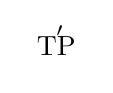
\begin{tikzpicture}[baseline=(root.base)]

        \Tree 	[.\node(root){TP};
                    [.{DP2\tss{i}} \edge [roof];
                        {[as crianças]\tss{\emph{u}K[\Nom]}} ]
                    [.T$'$
                        T\tss{K[\Nom]}
                        [.VP
                            V
                            [.DP1 \edge [roof];
                                {[o dentinho t\tss{1}]\tss{\emph{u}K[\Nom]}} ]
                        ]
                    ]
                ]

    \end{tikzpicture}
    \z

C is then merged with TP, as in \eqref{ex:key:14.36} below, and its unvalued
φ-features probe DP2’s valued \isi{φ-features}. As a consequence, T inherits C’s
φ-features already valued, as represented below.

\ea%36
    \label{ex:key:14.36}
    \begin{tikzpicture}[baseline=(root.base)]

        \Tree   [.\node(root){CP};
                    C
                    [.TP
                        [.{DP2\tss{i}} \edge [roof];
                            {[as crianças]\tss{\emph{u}K[\Nom]}} ]
                        [.T$'$
                            T\tss{\emph{u}φ[\Tpl],K[\Nom]}
                            [.VP
                                V
                                [.DP1 \edge [roof];
                                    {[o dentinho t\tss{1}]\tss{\emph{u}K[\Nom]}} ]
                            ]
                        ]
                    ]
                ]

    \end{tikzpicture}
\z

Note that this derivation is also possible in cases in which DP2 is not a
modifier of DP1, but a locative adverbial adjunct modifying VP, as previously
exemplified in \eqref{ex:key:14.1}, reproduced in (\ref{ex:key:14.37}a) below.
In such sentences, DP2 \emph{as ruas do centro} ‘downtown streets’ is initially
adjoined to VP and, from this position, c-commands and can probe DP1
\emph{carro} ‘carro’ before it moves to SpecTP.\largerpage[1]

\ea%37
    \label{ex:key:14.37}
	\ea     As ruas do centro não tão passando carro.
    \ex     {}[\tss{TP} T [\tss{VP} [\tss{DP2} as ruas do centro ]\tss{\emph{u}K[Y]}
                [\tss{VP} [\tss{V$'$} V [\tss{DP1} carro ]\tss{\emph{u}K[Y]} ]]]]
    \z
\z

A prediction of this analysis is that also in EP, DP2 and DP1 can share a Case
feature, which implies that in sentences with \isi{possessor raising} like
\eqref{ex:key:14.33}, DP2 can be moved from inside DP1 without a preposition, as in
BP. But, in contrast with BP, DP2 cannot be internal-merged as SpecTP in EP,
which explains why DP2 does not agree with T’s φ-feature\is{φ-features} in the European
variety. This fact is captured by our proposal, since SpecTP in \gls{EP}\il{European Portuguese} can
only be created after T inherits the unvalued \isi{φ-features} from C\@: in this
configuration, what determines the creation of SpecTP is a probe triggered by
C--T’s unvalued \isi{φ-features}, which means that SpecTP is a typical A-position in
\gls{EP}\il{European Portuguese}; as DP1 is locally closer to T than DP2 to satisfy φ-feature\is{φ-features}
requirements, only the former can be detected by the probe and internal-merged
as SpecTP\@.  However, the prepositionless DP2 can be moved to a topic position
in \gls{EP}\il{European Portuguese} (given that such \isi{movement} does not involve locality conditions
determined by φ-feature\is{φ-features} requirements), as well as in BP, as in \eqref{ex:key:14.38}
below (cf.\ \citealt{Costa2010} and \citealt{AvelarGalves2011}).

\ea%38
    \label{ex:key:14.38} \gls{BP}\il{Brazilian Portuguese}: ok -- \gls{EP}\il{European Portuguese}: ok
    \ea
    \gll    As crianças, nasceu o dentinho.\\
            the children born.\Tsg{} the tooth\\
    \glt
    \ex     {}[\tss{TopP} [\tss{DP} as crianças ]\tss{i} Top [\tss{TP} pro\tss{\Expl} T [\tss{VP} nasceu [\tss{DP} o dentinho t\tss{i} ]]]]\\
            ‘About the children, their teeth are born.’
    \z
\z

With regard to \isi{hyper-raising} constructions,
\citeauthor{AvelarGalves2011}' (\citeyear{AvelarGalves2011,AvelarGalves2016})
explanation is preserved in this new proposal: since SpecTP is an A-bar
position in BP, \isi{movement} from a position within the embedded clause (SpecTP,
SpecTopP or SpecCP) to the matrix SpecTP is always licensed. Even though we
consider that the uninterpretable instances of Case feature are deleted during
or at the end of the embedded clause phase, all DPs from the embedded clause
are, in BP, available to be moved to the matrix T and probed by C--T’s
\isi{φ-features} (since it occupies an escape hatch position in the lower
phase).  Note that not only external argument DPs can be raised from embedded
clauses, but also internal arguments, as in \eqref{ex:key:14.39}, and even
non-argumental phrases (cf.\ \eqref{ex:key:14.5}).

\ea\label{ex:key:14.39}Brazilian Portuguese\\
    \gll    Esses  livros\tss{i} parecem que a biblioteca ainda não catalogou t\tss{i}.\\
            these books seem.\Tpl{} that   the library yet not catalogued.\Tsg{}\\
    \glt    ‘It seems that the library haven’t catalogued these books yet.’
\z

\section{Prepositional locative subjects, pronominal morphology and
active-passive alternation}\label{sec:key:14.6}

\textcite{AvelarGalves2011,AvelarGalves2016} do not consider the case of
\eqref{ex:key:14.3}, reproduced in \eqref{ex:key:14.40} below, in which the verb
is preceded by a locative PP.

\ea%40
    \label{ex:key:14.40}Brazilian Portuguese\\
    \gll    \textbf{Na} \textbf{minha} \textbf{escola} aceita {cartão de crédito}.\\
            in-the my school accept.\Tsg{} {credit card}\\
    \glt    ‘My school accepts credit cards.’\\
            ‘One accepts credit cards in my school.’
\z

\citet{AvelarCyrino2008} give arguments that this locative PP behaves like a
subject, which led the authors to assume that it occupies SpecTP. According to
\citet{Avelar2006}, some instances of locative PPs in \gls{BP}\il{Brazilian Portuguese} can be analyzed
as projections of an adverbial pronoun, which can be phonologically null or be
spelled-out as an adverbial demonstrative like \emph{aqui} ‘here’ or
\emph{aí/ali/lá} ‘here’, as in the bracketed phrase in \eqref{ex:key:14.41}. Since
these adverbs have a (pro)nominal nature, locative PPs are, in fact, nominal
constituents in \gls{BP}\il{Brazilian Portuguese} sentences exemplified in \eqref{ex:key:14.40} above.
Then, such PPs are projections of a null adverbial pronoun with an unvalued
Case feature. In order to distinguish a nominal locative PP from a true PP, we
will call it LocP, whose head is the null locative adverbial pronoun
(pro\tss{\Loc}).

\ea\label{ex:key:14.41}
    \gll    [ (Aqui / {Aí / Ali / Lá)} na minha escola ] aceita {cartão de crédito}\\
            {} \hphantom{(}here {} there in-the my school {} accepts {credit card}\\
\z

Assuming that this analysis is on the right track, a logical step forward is
the claim that, in sentences like \eqref{ex:key:14.41}, no null subject\is{null subjects} is present
in the TP layer. It is likely to be the case that no null subject\is{null subjects} is present at
all. This means that the external argument of the verb is completely absent
from the derivation, and no \emph{v}P is projected. LocP is initially adjoined
to SpecVP, as a locative modifier constituent. If this is true, the Case
feature of LocP, present in the null adverbial pronoun, can probe the unvalued
Case feature of the DP \emph{cartão de crédito} ‘credit card’, which
results in feature sharing. LocP is then moved to T and probes the valued Case
feature of T. As a consequence, both LocP in SpecTP and the DP in complement
position are marked as nominative\is{nominative case} by Case-agreement with T.

\ea\label{ex:key:14.42}
    \ea {}[\tss{VP} [\tss{LocP} pro\tss{\Loc} na minha escola ]\tss{\emph{u}K[Y]}
            [\tss{VP} V [\tss{DP} cartão de crédito]\tss{\emph{u}K[Y]} ]]
    \ex {}[\tss{TP} [\tss{LocP} pro\tss{\Loc} na minha escola ]\tss{\emph{u}K[\Nom]}
            [\tss{T$'$} T\tss{\emph{u}K[\Nom]} [\tss{VP} t [\tss{VP} V
                [\tss{DP} cartão de crédito]\tss{\emph{u}K[\Nom]}
    \z
\z

Evidence that the post-verbal DP receives nominative\is{nominative case} Case is found in the
contrast between \eqref{ex:key:14.43} and~\eqref{ex:key:14.44} below. In
\eqref{ex:key:14.43}, the DP \emph{o hospital} is the external argument of the
verb \emph{tratar} ‘to treat’, and bears the nominative\is{nominative case} case. The second person
pronoun \emph{você} ‘you’ is the internal argument of the verb and its Case is
valued as accusative. In this case, the second person pronoun can be realized
as a clitic, with the form \emph{te}, as in (\eqref{ex:key:14.43}b). The
\emph{você}/\emph{te} variation, however, is not possible in
\eqref{ex:key:14.44}, in which the LocP \emph{no hospital} occupies SpecTP, as
in the analysis for the sentence in \eqref{ex:key:14.41}
and~\eqref{ex:key:14.42} above. The agrammaticality of (\eqref{ex:key:14.44}b) is
what our analysis predicts if the post-verbal DP is nominative\is{nominative case} in this
construction: only \emph{você} is compatible with nominative\is{nominative case} Case, since the
clitic pronoun \emph{te} is either accusative or dative\is{dative case}.

\ea\label{ex:key:14.43}Brazilian Portuguese
    \ea
    \gll    O hospital trata você bem.\\
            the hospital treats you well\\
    \ex
    \gll    O hospital te trata bem.\\
            the hospital you.\Acc{} treats well\\
    \glt    ‘Hospitals take care of you well.’
    \z
\z

\ea\label{ex:key:14.44}Brazilian Portuguese
    \ea[]{
	\gll    No hospital trata você bem.\\
            in-the hospital treats you well\\}
    \ex[*]{
    \gll    No hospital te trata bem.\\
            in-the hospital you.\Acc{} treats well\\
    \glt    ‘In hospitals one takes care of  you  well’}
    \z
\z

Things are different if the verb bears a plural mark, as in
\eqref{ex:key:14.45}, which yields a referentially indeterminate interpretation
for the subject: in this case, the variation between \emph{você} and \emph{te}
is again possible. This is because there is a null external argument (an
indefinite third plural person \emph{pro}) that bears nominative\is{nominative case} Case, and the
pronoun in complement position is accusative.


\ea\label{ex:key:14.45}Brazilian Portuguese
    \ea
	\gll    No hospital tratam você bem.\\
            in-the hospital treat.\Tpl{} you well\\
    \ex
    \gll    No hospital te tratam bem.\\
            in-the hospital you.\Acc{} treat.\Tpl{} well\\
    \glt    ‘In hospital, they treat you well.’
    \z
\z

The proposed analysis explains the difference in the interpretation of the
third person singular and plural with no phonologically explicit subject. We
straightforwardly derive it from the fact that only when the verb has plural
number does a null subject\is{null subjects} really occur.\footnote{In generic
    sentences with no pre-verbal DP or PP, like \emph{Não usa mais saia} ‘One
no longer wears skirts.’, we suggest that SpecTP is occupied by a null locative
expletive\is{expletives}, equivalent to English ‘there’.} Sentences like
(\eqref{ex:key:14.44}a) have no null subject, and they are in fact a kind of
ergative sentences, in which the projected argument in complement position
bears nominative\is{nominative case} Case. If this argument remains
post-verbal, an extra position is available in SpecTP. It can be occupied by a
LocP/PP like in (\eqref{ex:key:14.44}a), or by the verbal complement, like in
\eqref{ex:key:14.46} below. In the latter, also impossible in EP, the verbal
complement \emph{a revista} ‘the journal’ is attracted to SpecTP, where it
Case-agrees with T, as represented in \eqref{ex:key:14.47}.

\ea\label{ex:key:14.46}Brazilian Portuguese\\
    \gll    A revista xerocou.\\
            the journal photocopied.\Tsg{}\\
    \glt    ‘The journal was photocopied.’
\z

\ea\label{ex:key:14.47}
    {}[\tss{CP} C [\tss{TP} [\tss{DP} a revista ]\tss{φ[\Tsg{}]/K[\Nom]} [\tss{T$'$} T\tss{φ[\Tsg]/K[\Nom]}  [\tss{VP} V t ]]]]
\z

The hypothesis that no external argument is projected in \eqref{ex:key:14.44} and
\eqref{ex:key:14.46} is reinforced by the fact that no adverbial phrase semantically
associated with an agentive argument can be inserted in this kind of sentences
(cf.\ \citealt{Galves2000}):

\ea%48
    \label{ex:key:14.48}Brazilian Portuguese
    \gll    \llap{\#}A revista xerocou \textbf{com} \textbf{cuidado} / \textbf{para} \textbf{ganhar} \textbf{tempo}.\\
            the journal photocopied.\Tsg{} with care {} to gain time\\
\z

Finally, we have to account for the variation in morphological agreement
be\-tween the verb and its subject (cf.\ iv in \Cref{sec:key:14.2}), which was
linked with the presence or absence of Case feature on DPs in the former
analysis (cf.\ \Cref{sec:key:14.4.1}). In the present analysis, the possibility
of no agreement on the verb is no longer imputable to the absence of
Case-feature on the subject DP. An alternative analysis comes from the
parallelism that can be done between the nominative--dative alternation attested
in pronominal subjects of embedded infinitival sentences (cf.\
\eqref{ex:key:14.21}) and the alternation involving agreement and no-agreement
in tensed sentences.

Regarding embedded infinitival clauses, as exemplified in \eqref{ex:key:14.49}
below, the analysis proposed in this paper yields two different derivations
according to whether non-finite Tense has or not a Case feature. This is a
possibility in \gls{BP}\il{Brazilian Portuguese} as well as in EP, since both
varieties license inflected infinitives \parencite{Raposo1987,Modesto2016}.
Like in tensed sentences, T’s \gls{EPP}\is{Extended Projection Principle} of infinitival sentences attracts the
external argument to SpecTP. There are then two possibilities in BP, according
to whether T has Case or not. If T has Case, as represented in
(\ref{ex:key:14.51}a), DP in SpecTP probes it, and is marked as nominative\is{nominative case}. If
T does not have Case, as in (\ref{ex:key:14.50}b), DP in SpecTP can receive
dative Case from the preposition \emph{para} ‘for’, and then be spelled-out as
the oblique pronoun \emph{mim} ‘me’.\footnote{It is not clear for us how the
    pronoun in SpecTP receives its dative\is{dative case} Case from the preposition \emph{para}
    ‘for’ within \citegen{PesTor2004} proposal. A possible analysis is that
dative Case is transferred from the preposition (which may be in C) to
non-inflected T, and then be probed by the pronoun. A full account of this
question is outside the scope of this paper.} Both derivations can be derived
from the basic assumption of our analysis, i.e. the fact that DPs are moved to
SpecTP before the merge of C into the structure.\footnote{This assertion is not
    true in the case of null subjects as we discuss
    below.}\textsuperscript{,}\footnote{In \gls{EP}\il{European Portuguese},
    the pronominal external argument is probed by T and internal-merged to
    SpecTP only after T receives \isi{φ-features} from C. In non-inflected/impersonal
    infinitival clauses, C does not have \isi{φ-features} to be inherited by T, and
the pronoun cannot be moved to SpecTP.  As a consequence, the pronoun cannot
probe T’s Case feature and does not receive nominative\is{nominative case} Case, which yields an
ungrammatical sentence.}

\ea%49
    \label{ex:key:14.49}Brazilian Portuguese\\
    \gll    Ele fez isso pra mim / eu ficar feliz.\\
            He did that for me {} I to.stay happy\\
    \glt    ‘He did that to make me happy’
\z

\ea%50
    \label{ex:key:14.50}
	\ea
    {}[\tss{CP} pra\tss{K[\Dat]} [\tss{TP} [ \Fsg{} = \textbf{eu} ]\tss{K[\Nom]}
        [\tss{T$'$} T\tss{φ[\Fsg],K[\Nom]} [\tss{VP} ficar feliz ]]]]
    \ex
    {}[\tss{CP} pra\tss{K[\Dat]} [\tss{TP} [ \Fsg{} = \textbf{mim} ]\tss{K[\Dat]}
        [\tss{T$'$} T [\tss{VP} ficar feliz ]]]]
    \z
\z

Regarding the variation in subject--verb agreement\is{agreement!subject
agreement} in finite sentences, we can explore two possibilities involved in
the C--To-T transfer of features. In our proposal, since SpecTP is already
created when C is connected into TP, φ-features can be transferred valued to T
in BP. The two possibilities are then the following: (i) C transfers its valued
\isi{φ-features} to T, or (ii) C retains its \isi{φ-features}. The situation in
(i) produces sentences in which the morphological mark of agreement is on the
verb, as in \eqref{ex:key:14.51}.  In the second situation, C cannot be
morphologically inflected in BP, and the verb is spelled-out with the default
mark of third singular person -- cf.\ \eqref{ex:key:14.52}.\footnote{But if the
    subject is the first singular person pronoun \emph{eu} ‘I’, agreement
    marking is obligatory in some tenses of indicative mode (Present, Future
    and Perfect). One possible hypothesis is that the obligatory agreement does
    not result from the syntactic C-To-T transfer, but from a morphological
    adjustment triggered by the presence of the first-person pronoun in the
    immediately preverbal position. A piece of evidence in favor of this
    hypothesis is the fact that, when the pronoun is phonologically null,
    agreement is no longer necessary in many conversational contexts.  For
    instance, a question like \emph{Você} \emph{fez} \emph{o} \emph{café?} ‘Did
    you make coffee?’ can be answered as in (ii), with the verb inflected in
    the third singular person if the subject pronoun is null. If the pronoun is
    inserted, the agreement is obligatory, as in (iii).

    \begin{exe}
        \exi{(i)}
        \gll    Eu falo / *fala.\\
                I speak.\Fsg{} {} \hphantom{*}speak.\Tsg{}\\
        \glt    ‘I speak.’
        \exi{(ii)}
        \gll    Fez / Fiz.\\
                made.\Tsg{} {} made.\Fsg{}\\
        \glt    ‘Yes, I made it.’
        \exi{(iii)}
        \gll    Eu (*fez) / fiz.\\
                I \hphantom{(*}made.\Tsg{} {} made.\Fsg{}\\
        \glt    ‘Yes, I made it.’
    \end{exe}}

\ea%51
    \label{ex:key:14.51}Brazilian Portuguese
	\ea
	\gll    As crianças dormiram.\\
            the.\Pl{} children slept.\Tpl{}\\
    \glt    ‘The children slept.’
    \ex
        {}[\tss{CP} C [\tss{TP} [\tss{DP} as crianças ]\tss{φ[\Tpl]}
            [\tss{T$'$} T\tss{φ[\Tpl]}[\tss{\emph{v}--VP} \dots{} ]]]]
    \z
\z

\ea%52
    \label{ex:key:14.52}Brazilian Portuguese
	\ea
	\gll    As crianças dormiu.\\
            the.\Pl{} children slept.\Tsg{}\\
    \glt    ‘The children slept.’
    \ex
        {}[\tss{CP} C\tss{φ[\Tpl]} [\tss{TP} [\tss{DP} as crianças ]\tss{φ[\Tpl]}
            [\tss{T$'$} T\tss{} [\tss{\emph{v}--VP} \dots{} ]]]]
    \z
\z

The other property of \gls{BP}\il{Brazilian Portuguese} explained by the absence of Case in the former
analysis was the morphological invariance of personal pronouns. This can be
independently accounted for by the morphological reorganization of the
pronominal paradigm due to language contact (cf.\ \Cref{sec:key:14.3}), which
includes, among other things, the loss of the third person clitic, and the
variation between second person clitic and its non-clitic counterpart. In
particular, a consequence of the loss of the accusative clitic is that
accusative non-clitic pronouns emerge in the paradigm. Third person pronoun
\emph{ele} ‘he’ and second person pronoun \emph{você} ‘you’ can therefore be
either nominative\is{nominative case} or accusative.  A full account of this question is outside
the scope of this paper.

\section{Concluding remarks}\label{sec:key:14.7}

The analysis proposed here departs from our previous accounts of Brazilian
mor\-pho\-syn\-tax in what concerns Case. In
\textcite{AvelarGalves2011,AvelarGalves2016}, we argued that DPs could enter
the derivation with or without a Case feature. This accounted for the free
variation between agreement and non-agreement with subjects, on the one hand, and
between tonic pronouns and \isi{clitics} on the other hand. It also accounted for the
fact that sentences with topic--verb agreement, like the ones in
\eqref{ex:key:14.1} and \eqref{ex:key:14.2}, seem to have only one source of
Case for two DPs.  Moreover, this was likely to be a nice claim from the
contact effects with African languages since it has been argued that syntactic
Case in \ili{Bantu} languages is not active (cf.\ \citealt{Diercks2012}). We gave
this hypothesis up for two main reasons. On the one hand, we are forced to
acknowledge the fact that BP displays many of the morphosyntactic properties
classically associated with abstract Case\is{case!abstract Case} (or
\emph{Vergnaud licensing} in \citegen{SheevanderWal2018} proposal).  On the
other hand, recent papers convincingly argued that not all \ili{Bantu}
languages lack the effects of syntactic case (cf.\ \citealt{vanderWal2015} and
references therein), which makes \citegen{AvelarGalves2011} proposal for
\gls{BP}\il{Brazilian Portuguese} less attractive from a diachronic point of
view.

One of the advantages of the new approach is also that Case and \gls{EPP}
nicely combine to account for the facts, while they were rather disconnected in
the previous analysis. Assuming feature sharing as in \citegen{PesTor2004}
proposal, we derive the constructions with topic--verb agreement from the way
Case and \isi{φ-features} interact with the ability of T in BP to enter in
nominative-Case-valuing with both the pre-verbal DP that c-commands it and the
post-verbal DP c-commanded by it.  This nicely solves the question of one Case
source for two DPs.  As for the other facts that the lack of Case was intended
to account for, it is worth coming back to the connection between Case and
\isi{hyper-raising}. One of the tests proposed by \citet{SheevanderWal2018} involves
\isi{hyper-raising}, since it is largely assumed in minimalist approaches that only
DPs with valued Case-feature are frozen in place. The existence of
\isi{hyper-raising} has been therefore considered as an empirical argument against
the relevance of syntactic Case\is{case!syntactic Case} in languages in which it is observed (for \ili{Bantu}
languages, see \citealt{Diercks2012}). It is therefore important to stress that
our claim that Case is active in \gls{BP}\il{Brazilian Portuguese} grammar has
no consequences on our analysis of \isi{hyper-raising}, which we continue to derive
from the φ-independence of T’s \gls{EPP}\is{Extended Projection Principle} and the A-bar status of SpecTP
position in this Portuguese variety.

Some facts recently discussed in the literature about \ili{Bantu} languages seem to
support this analysis. \Citet[127]{vanderWal2015}, for instance, claims that
some \ili{Bantu} languages like \ili{Makhuwa} and \ili{Matengo} display many
phenomena showing that their grammar activate abstract case. In those
languages, for instance, the verb agrees with its post-verbal subject in
locative inversion, behaving therefore like \ili{Indo-European} languages with
respect to \citegen{Baker2008} Agreement parameter, i.e., evidencing
sensitiveness to nominative\is{nominative case} Case. Still, such languages have \isi{hyper-raising}
(hyper-agreement, in van der Wal’s terms).  The comparison between \ili{Bantu}
languages in which the verb agrees with the post-verbal subject and \ili{Bantu}
languages in which the verb agrees with the pre-verbal locative phrase, leads
one to question \citegen{Baker2008} claim that the Agreement Parameter is a
macro-parameter that distinguishes large families of languages. On the basis of
this data, and if our analysis can be extended to \ili{Bantu} languages, it rather
looks like a morphological micro-parameter involving the way in which the
φ-features are transferred in the C--T domain, in the spirit of
\citet{Ouali2008}.\footnote{For an implementation of Ouali’s ideas to explain
aspects of Brazilian syntax, see \citet{Toniette2013}.} We have claimed that in
BP, \isi{φ-features} are already valued when they are transferred to T.  One could
suggest that, in some languages, C is blind to the constituent in SpecTP and
transfers unvalued \isi{φ-features} to T. In this case, agreement is established with
the post-verbal subject.

Finally, we have proposed that part of the debated question of Case
parametrization has to be put at the level of the morphological realization of
Case. This is not new, as we know that languages differ with respect to the
presence vs. absence of morphological Case-marking on DPs.  BP is a language in
which there is intra-linguistic variation inside the pronominal paradigm,
possibly due to its history of contact.

\printchapterglossary{}

\section*{Acknowledgements}

This article was partially supported by FAPESP Grant 2012/06078-9 and CNPq
Grant 309764/2014-9. We warmly thank Ian Roberts for a very illuminating
discussion of the previous version of our analysis. We are also very grateful
to two anonymous reviewers for their comments and suggestions. Any remaining
shortcomings of this article are entirely our responsibility.

{\sloppy
\printbibliography[heading=subbibliography,notkeyword=this]
}

\end{document}
